

\section{Wolfram Language Algorithms}
\label{codes_wolfram}

\begin{figure}[h]
	\centering
		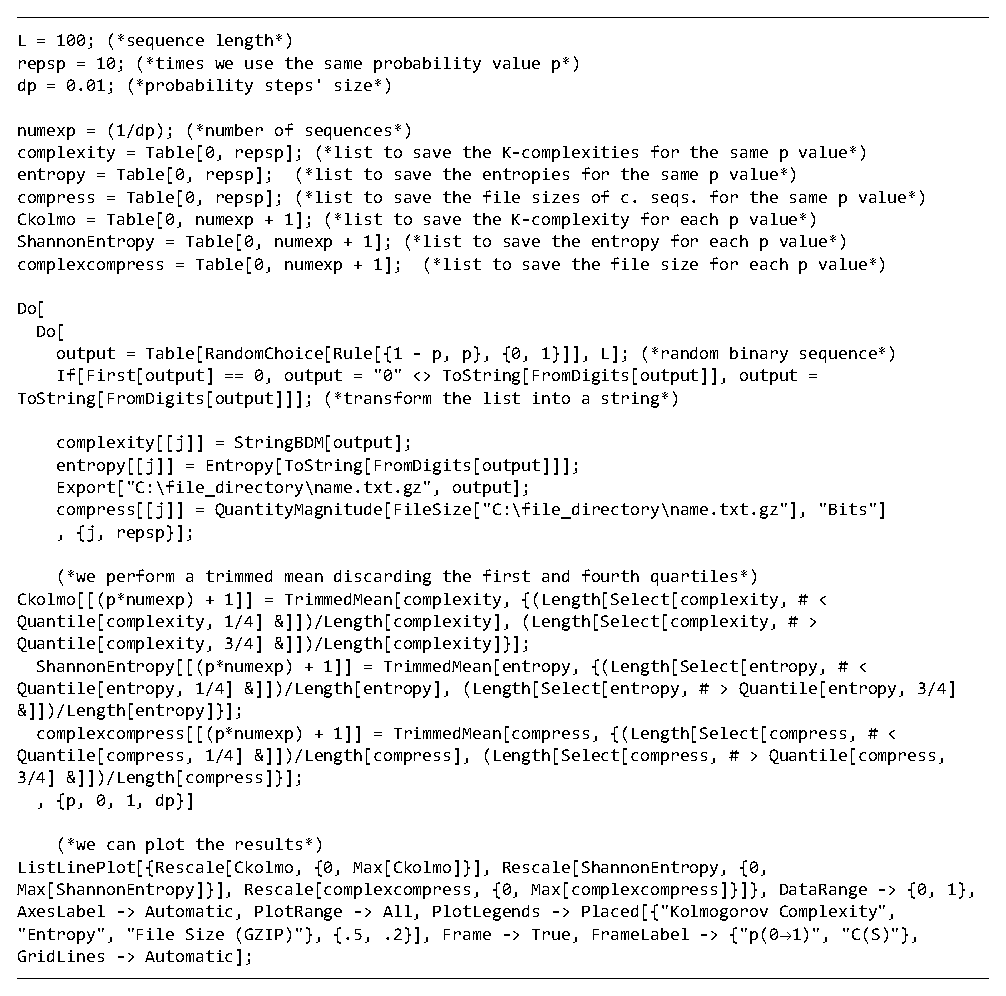
\includegraphics[width=\textwidth]{random_seqs}
	\caption{The code to generate and measure the complexity of random sequences of bits.}
	\label{fig:random_seqs_code}
\end{figure}

\begin{figure}[h]
	\centering
		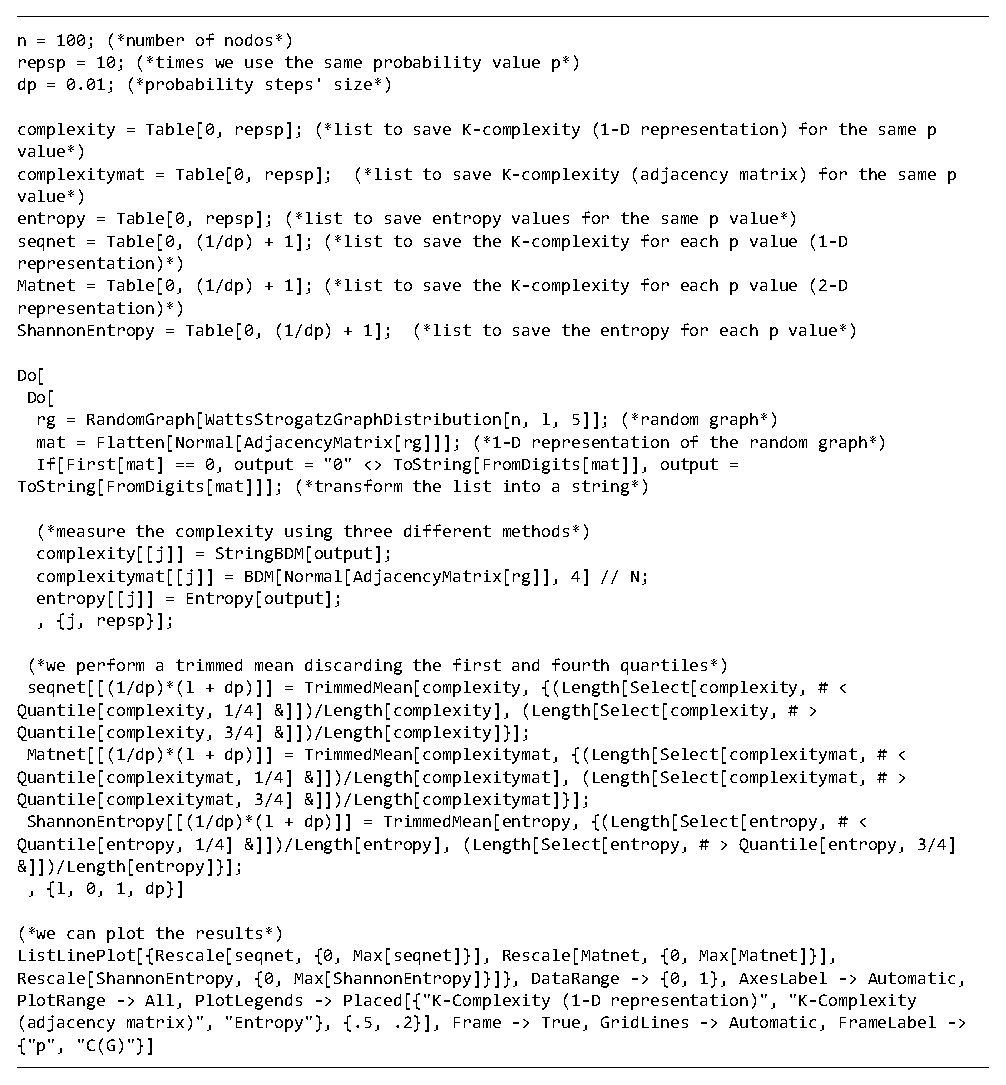
\includegraphics[width=\textwidth]{watts}
	\caption{The code to generate and measure the complexity of random graphs using the Watts-Strogatz graph distribution.}
	\label{fig:watts_code}
\end{figure}

\begin{figure}[h]
	\centering
		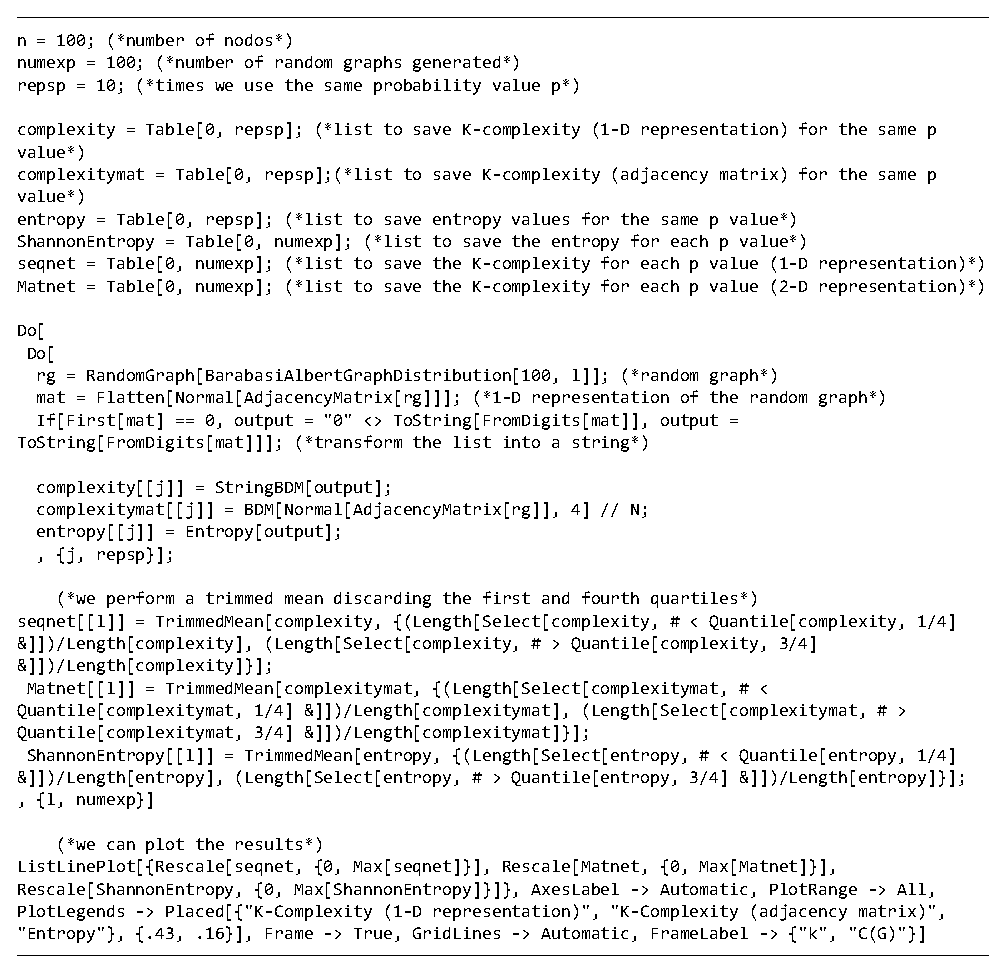
\includegraphics[width=\textwidth]{barabasi_code}
	\caption{The code to generate and measure the complexity of random graphs using the Barabási-Albert graph distribution.}
	\label{fig:barabasi_code}
\end{figure}

\begin{figure}[h]
	\centering
		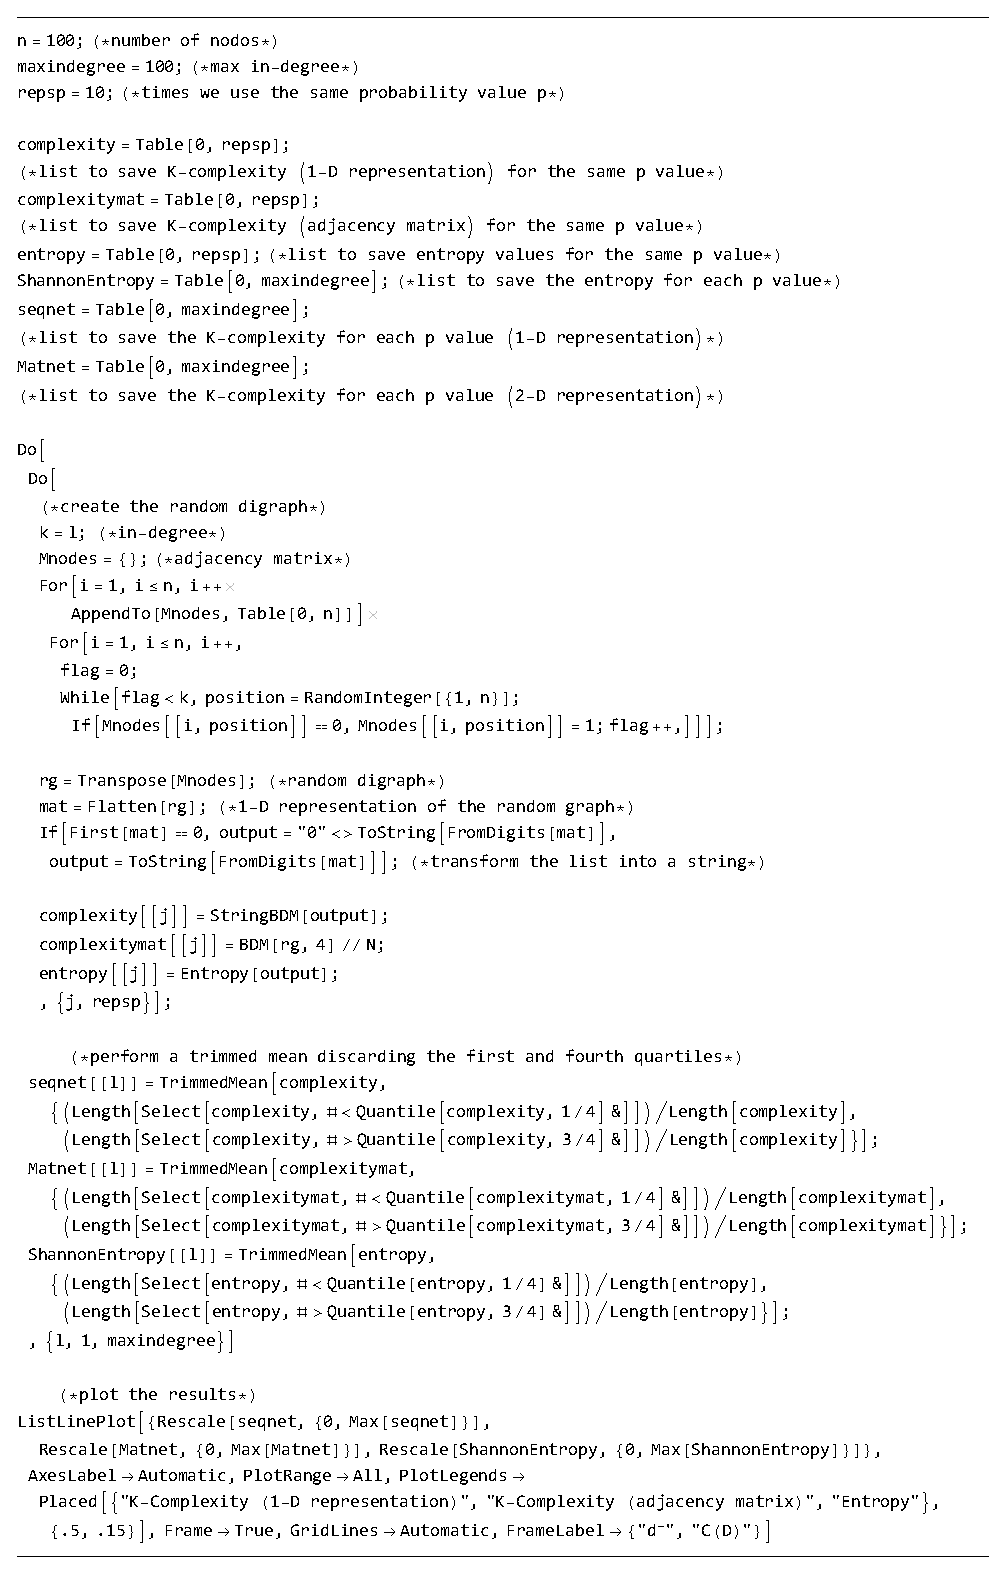
\includegraphics[width=\textwidth]{direc_aum_d_code}
	\caption{The code to generate and measure the complexity of random digraphs with increasing vertex in-degree.}
	\label{fig:direc_aum_d_code}
\end{figure}

\begin{figure}[h]
	\centering
		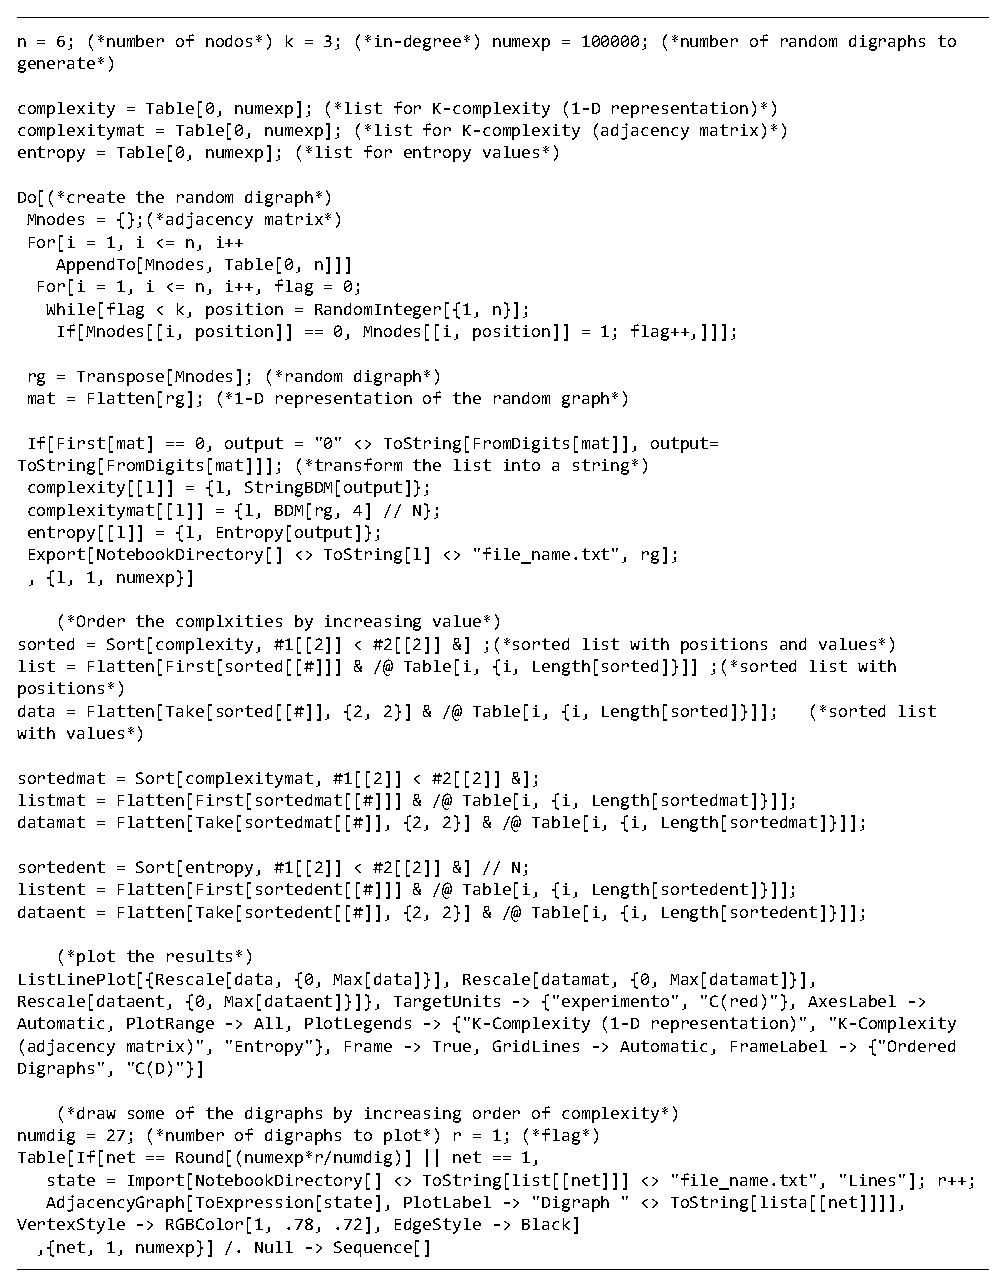
\includegraphics[width=\textwidth]{complex_di_k_cte_code}
	\caption{The code to generate and measure the complexity of random digraphs with a fixed number of nodes and in-degree.}
	\label{fig:complex_di_k_cte_code}
\end{figure}

\begin{figure}[h]
	\centering
		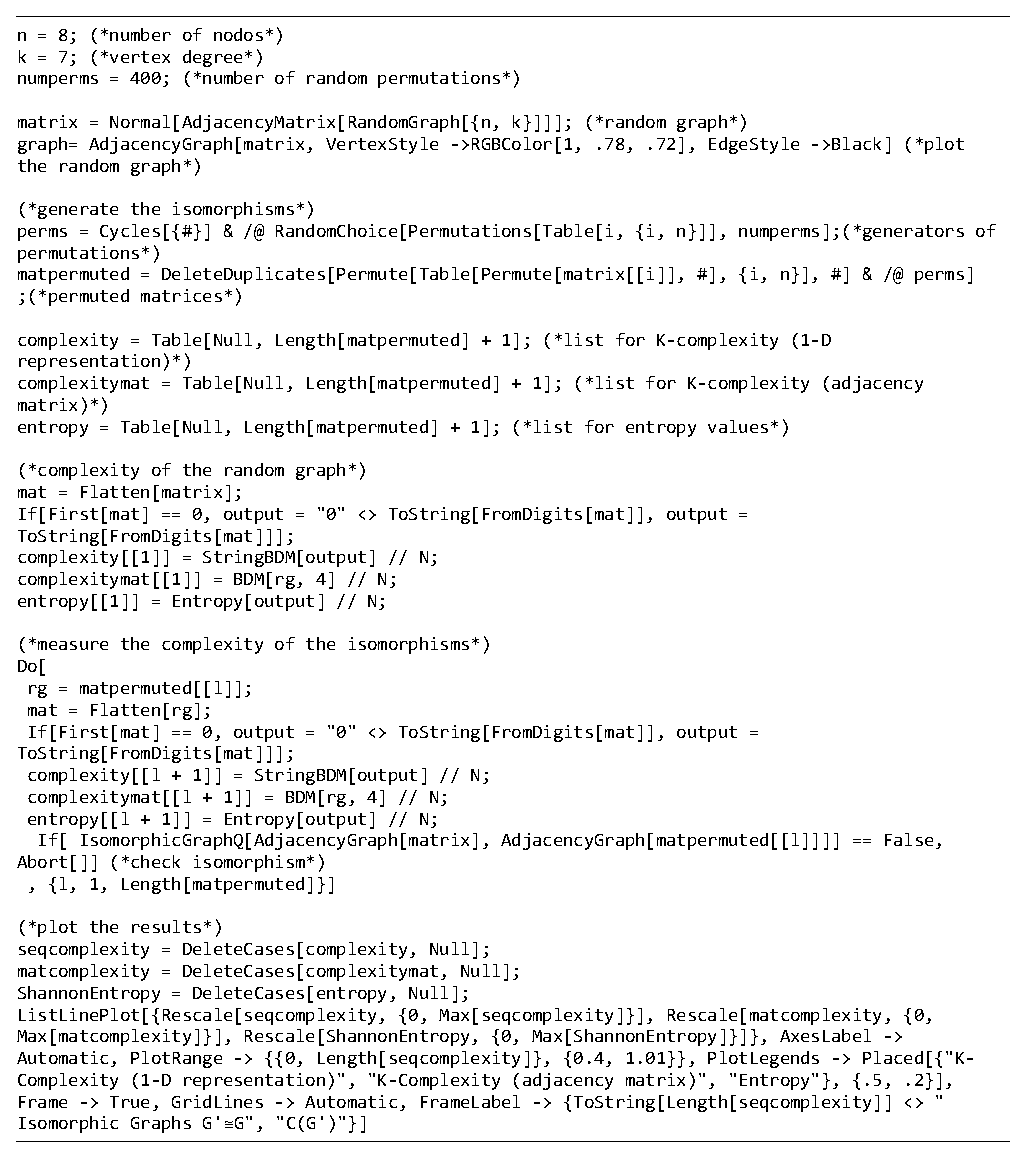
\includegraphics[width=\textwidth]{iso_G_code}
	\caption[The code to generate and measure the complexity of the isomorphisms of a random graph.]{The code to generate and measure the complexity of the isomorphisms of a random graph. To work with a random digraph of $n$ nodes and $k$ directed edges instead of a graph of $n$ nodes and $k$ edges, the argument \textit{DirectedEdges $\rightarrow True$} has to be added in the function \textit{RandomGraph}.}
	\label{fig:iso_G_code}
\end{figure}

\begin{figure}[h]
	\centering
		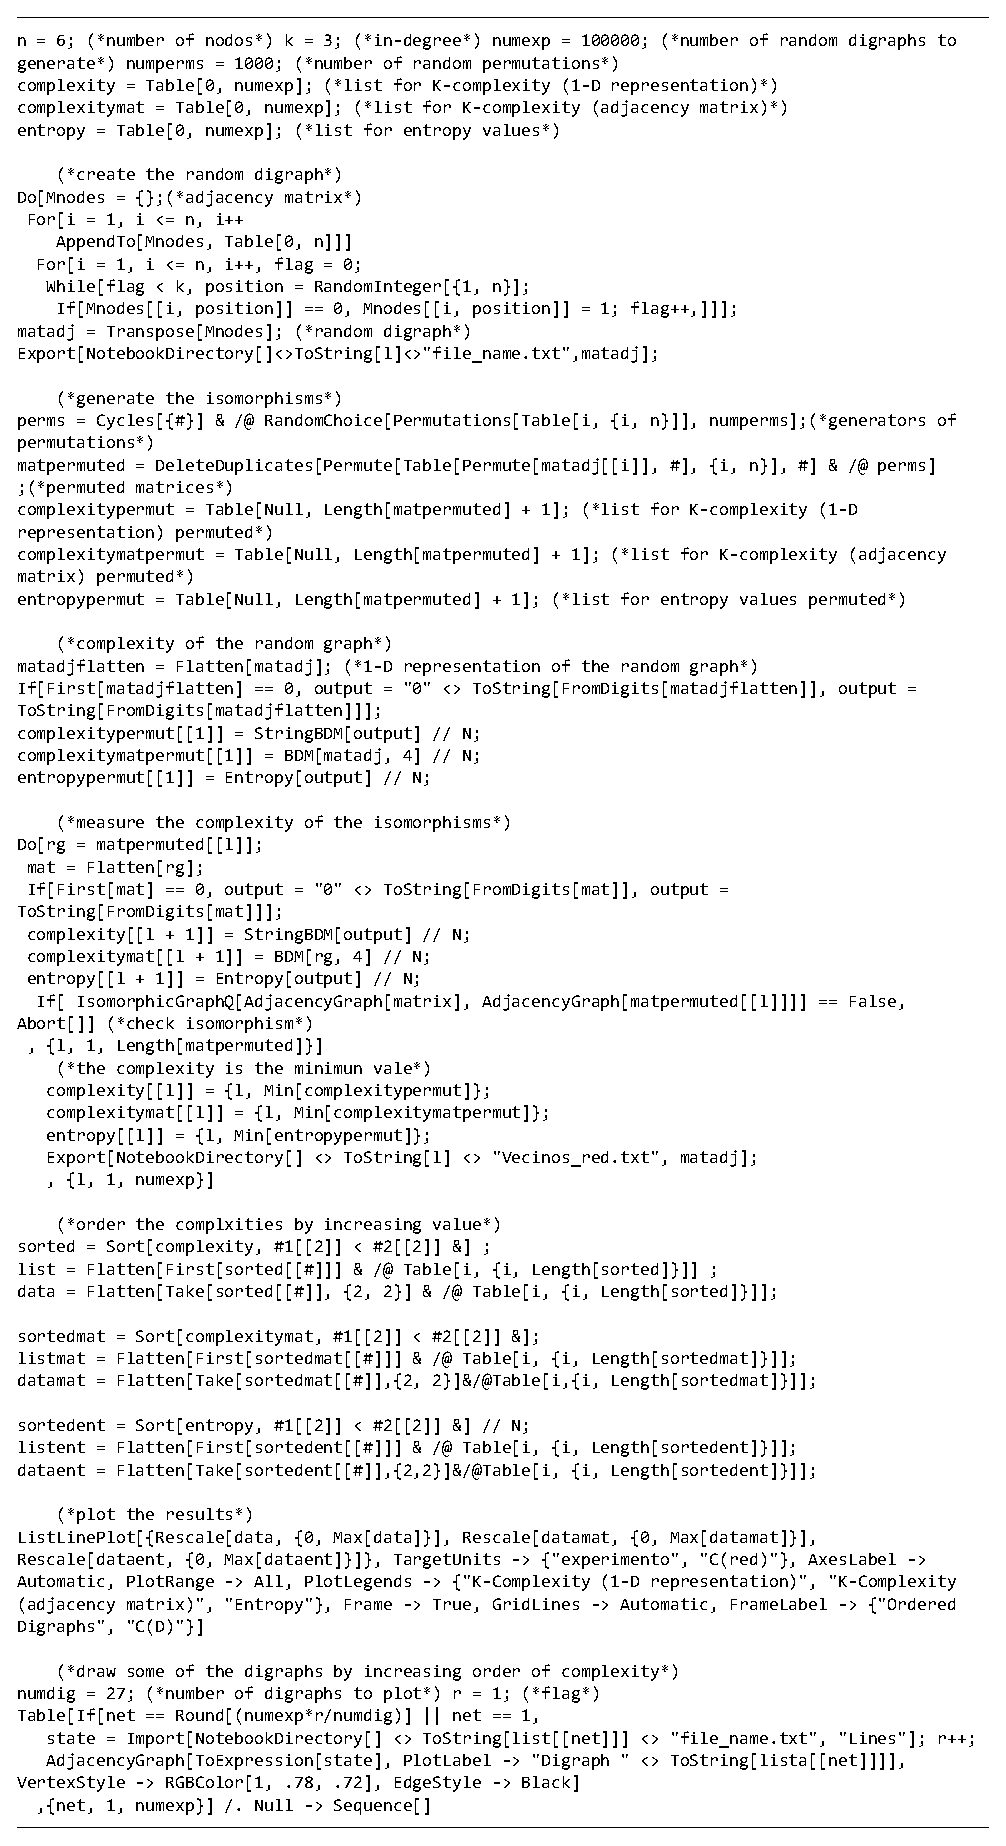
\includegraphics[width=\linewidth, height=\textheight,keepaspectratio]{iso_D_k_cte_code}
	\caption{The code to generate and measure the complexity of random digraphs with a fixed number of nodes and in-degree by considering its isomorphisms.}
	\label{fig:iso_D_k_cte_code}
\end{figure}

\begin{figure}[h]
	\centering
		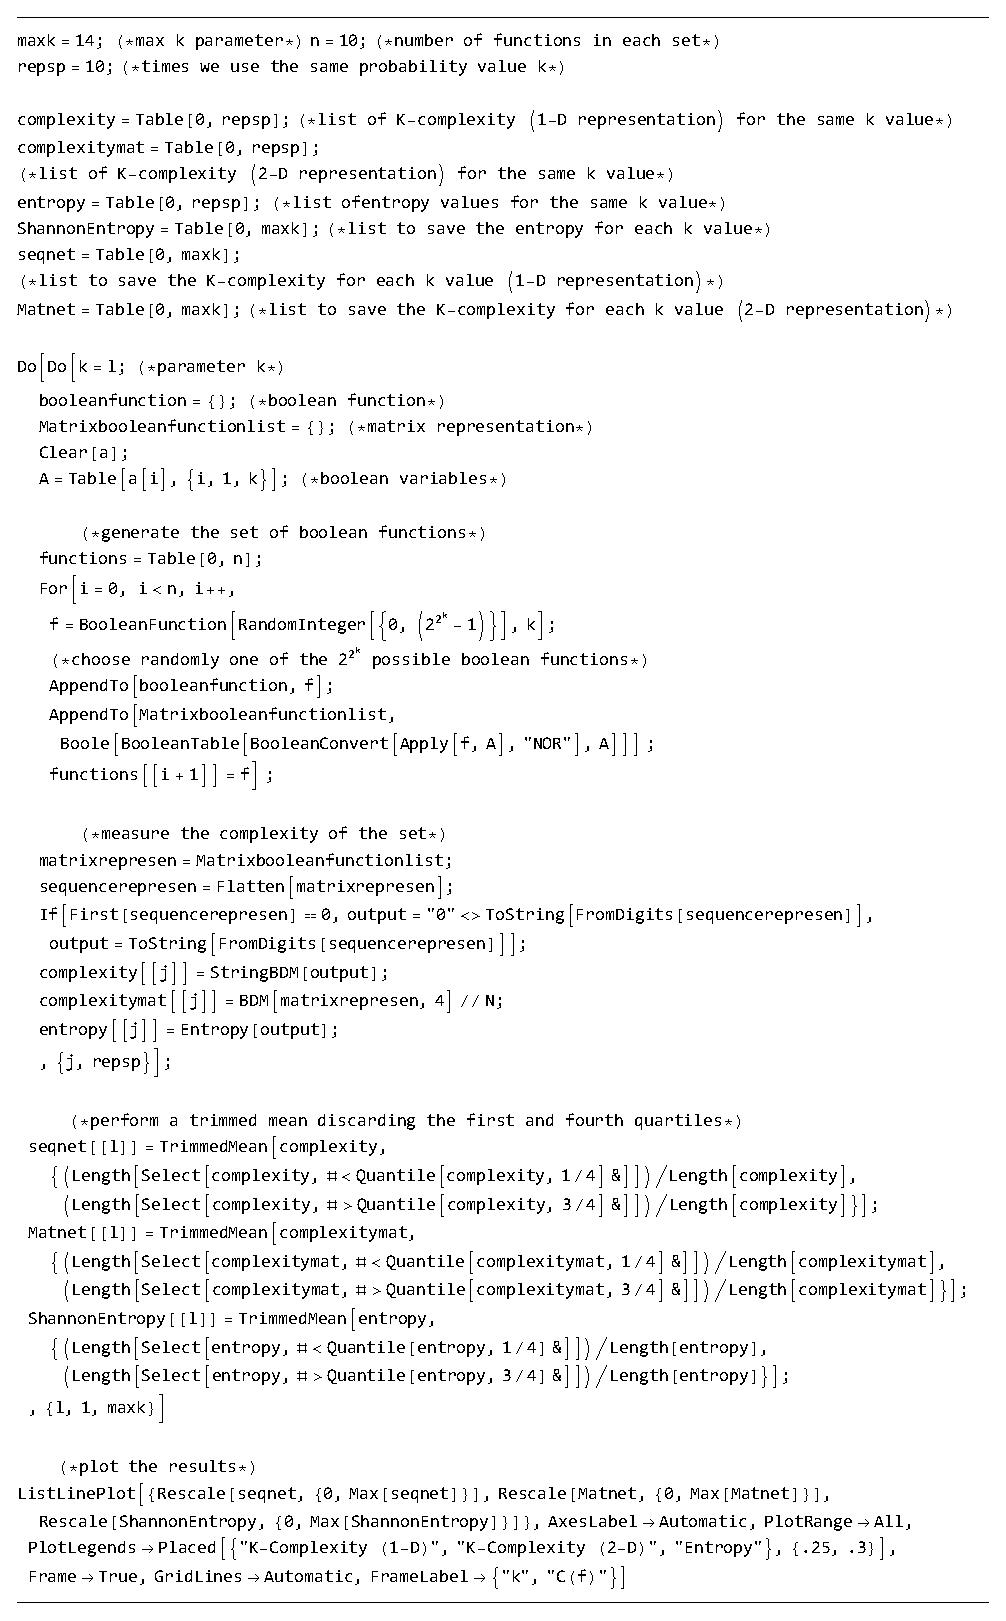
\includegraphics[width=\linewidth, height=\textheight,keepaspectratio]{set_bool_fun_k_inc_code}
	\caption{The code to generate and measure the complexity of random sets of boolean functions with increasing parameter $k$.}
	\label{fig:set_bool_fun_k_inc_code}
\end{figure}

\begin{figure}[h]
	\centering
		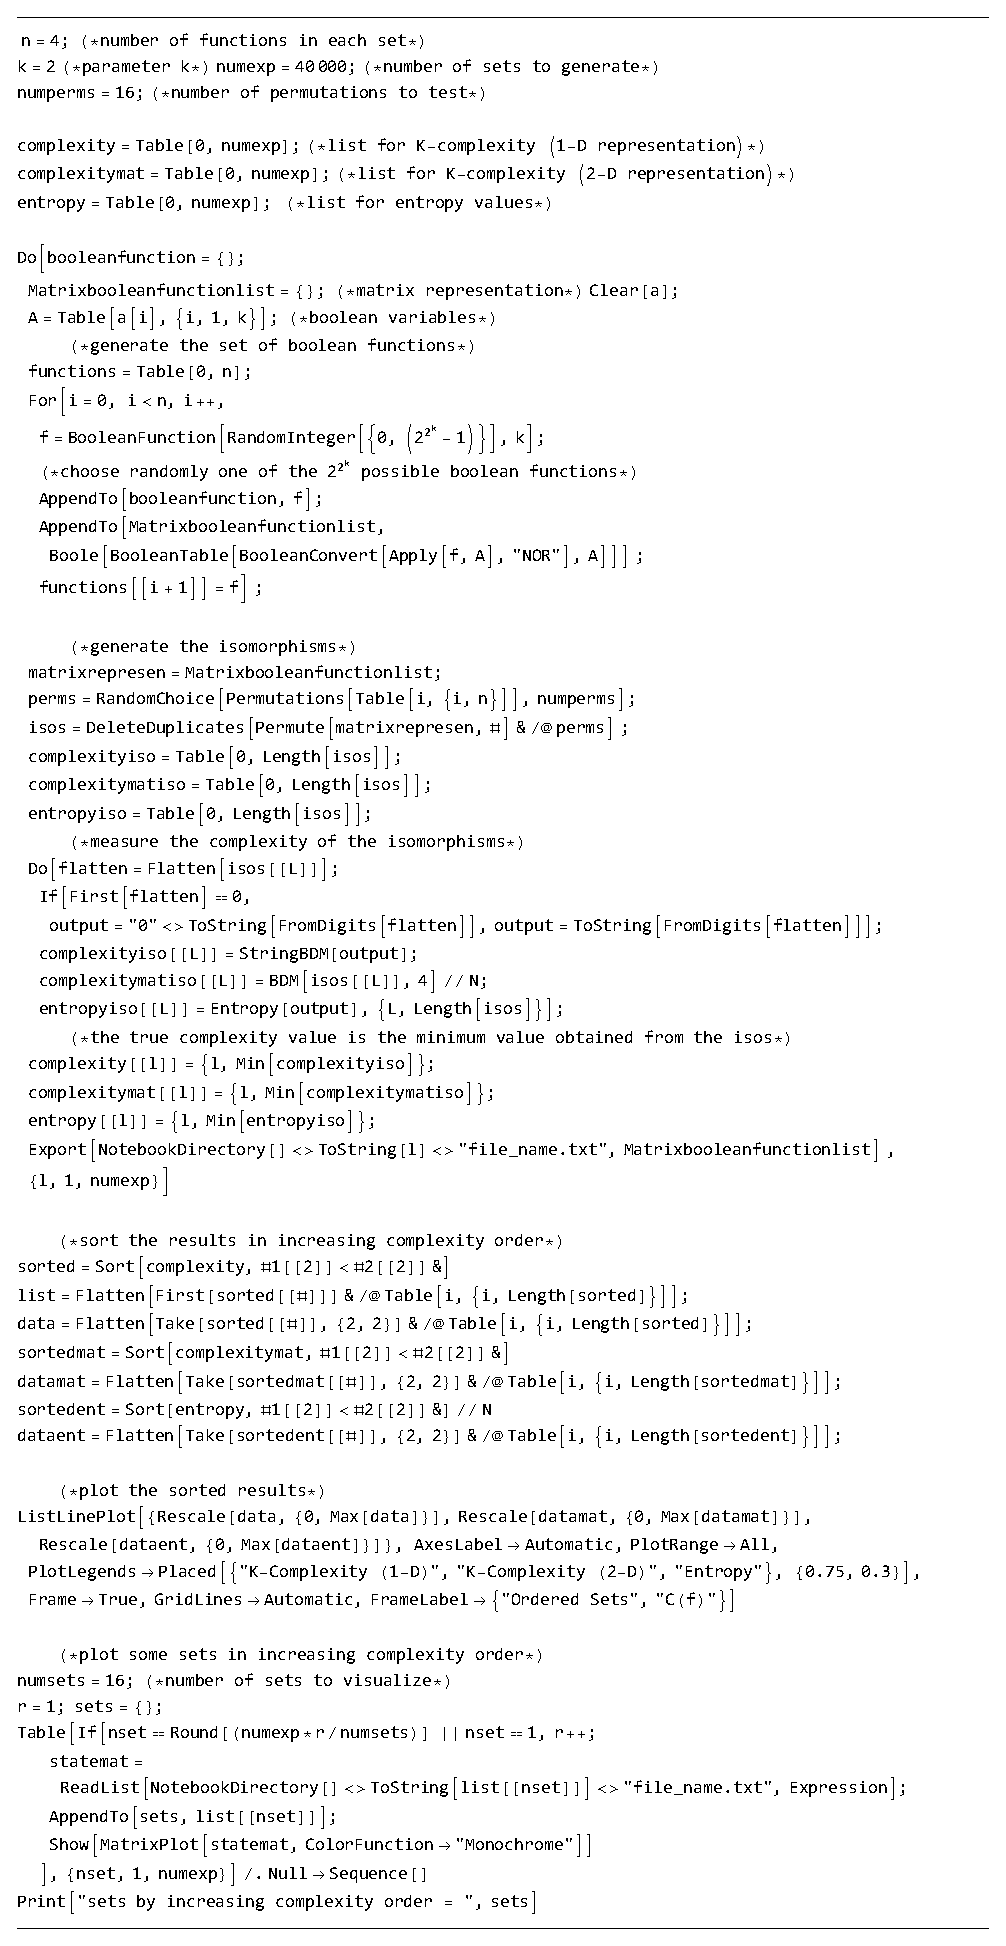
\includegraphics[width=\linewidth, height=\textheight,keepaspectratio]{set_bool_fun_code}
	\caption{The code to generate and measure the complexity of random sets of boolean functions with fixed parameter $k$ and $N$.}
	\label{fig:set_bool_fun_code}
\end{figure}

\begin{figure}[h]
	\centering
		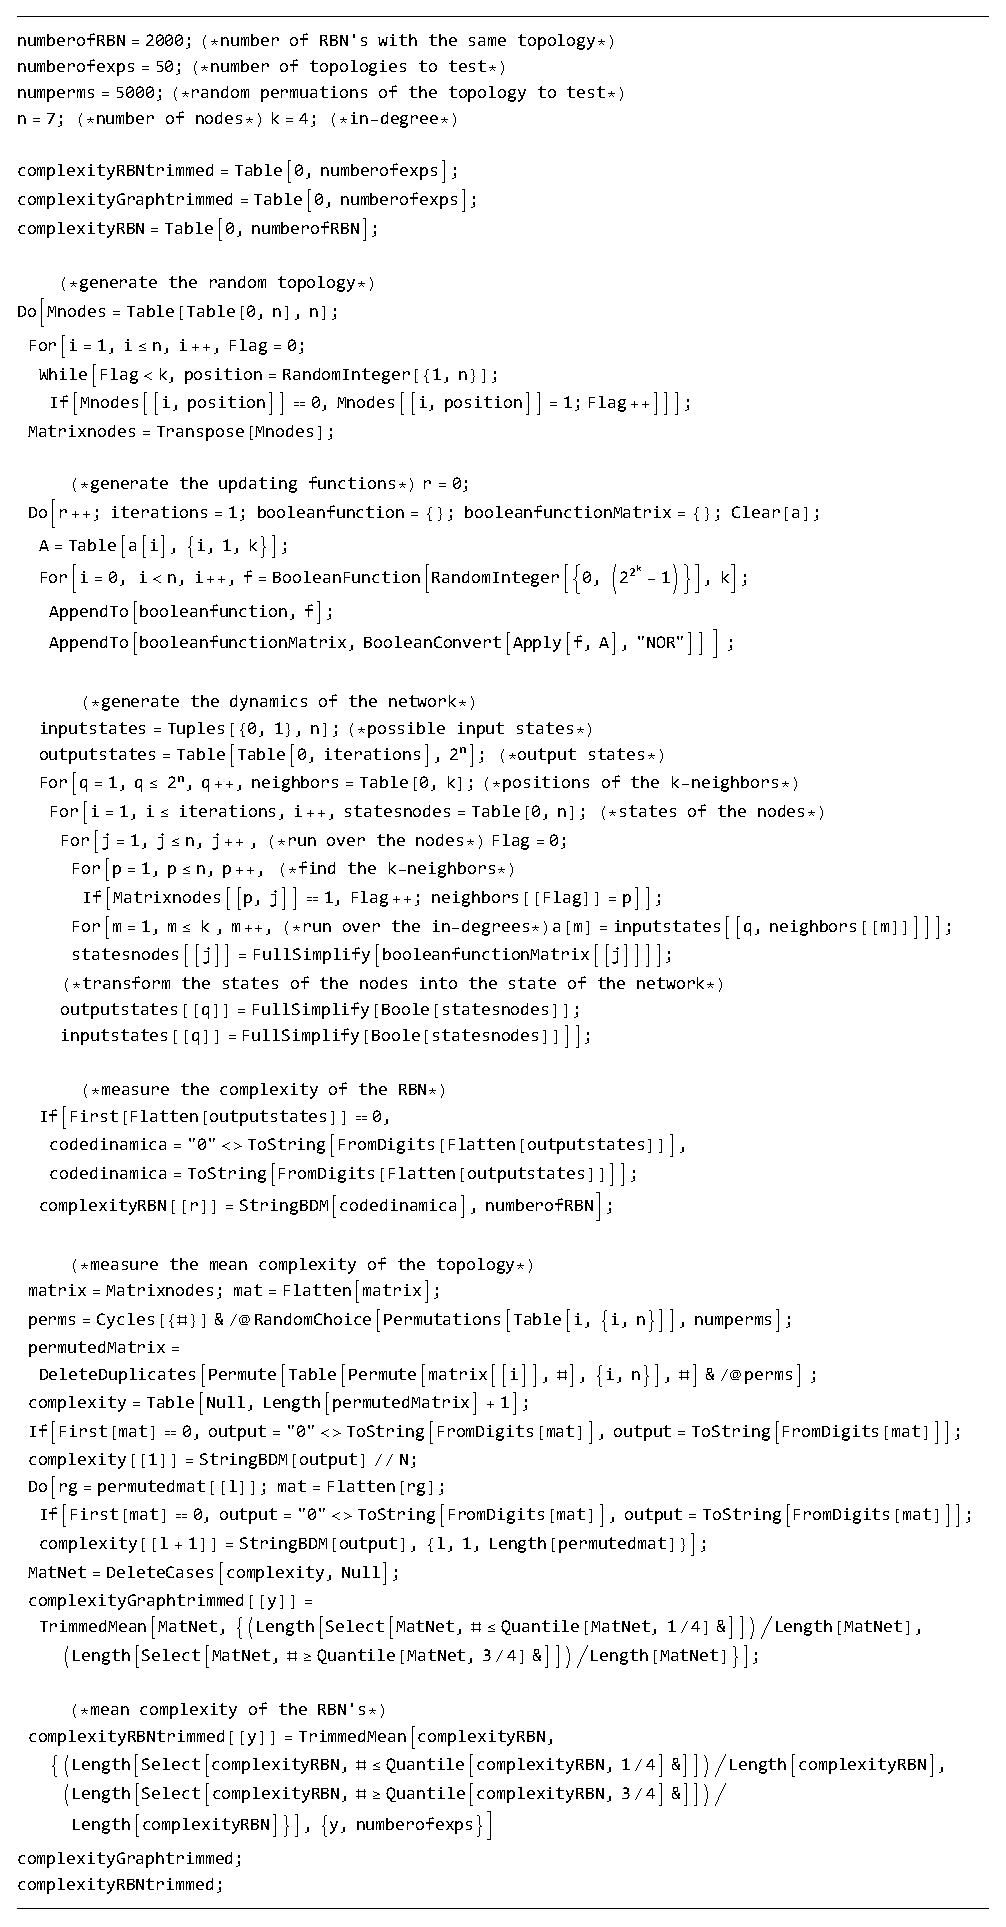
\includegraphics[width=\linewidth, height=\textheight,keepaspectratio]{rbn_vs_graph_complexity}
	\caption{The code to generate and measure the complexity of Random Boolean Networks which share the same topology.}
	\label{fig:rbn_vs_graph_complexity}
\end{figure}

\begin{figure}[h]
	\centering
		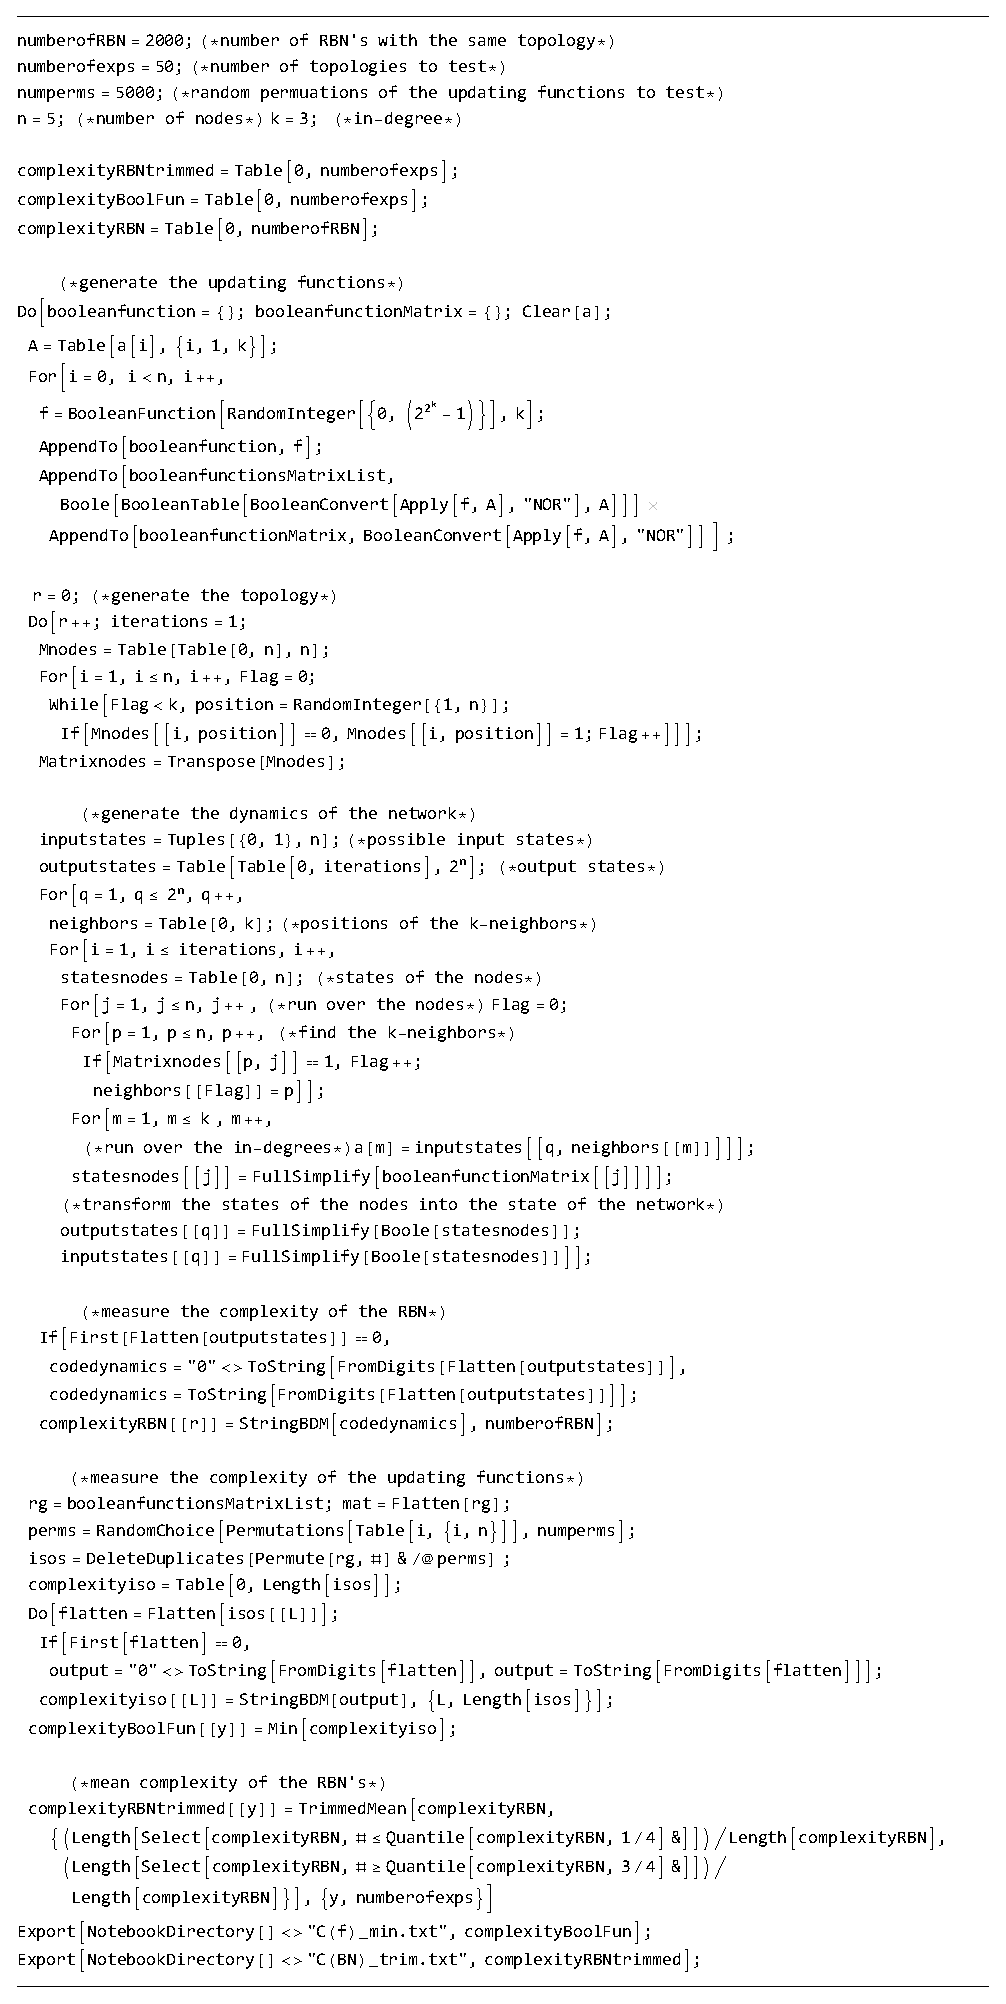
\includegraphics[width=\linewidth, height=\textheight,keepaspectratio]{rbn_vs_func_complexity}
	\caption{The code to generate and measure the complexity of Random Boolean Networks which share the same updating functions.}
	\label{fig:rbn_vs_func_complexity}
\end{figure}

\clearpage

\section{Python Algorithms}
\label{codes_python}

\begin{figure}[h]
	\centering
		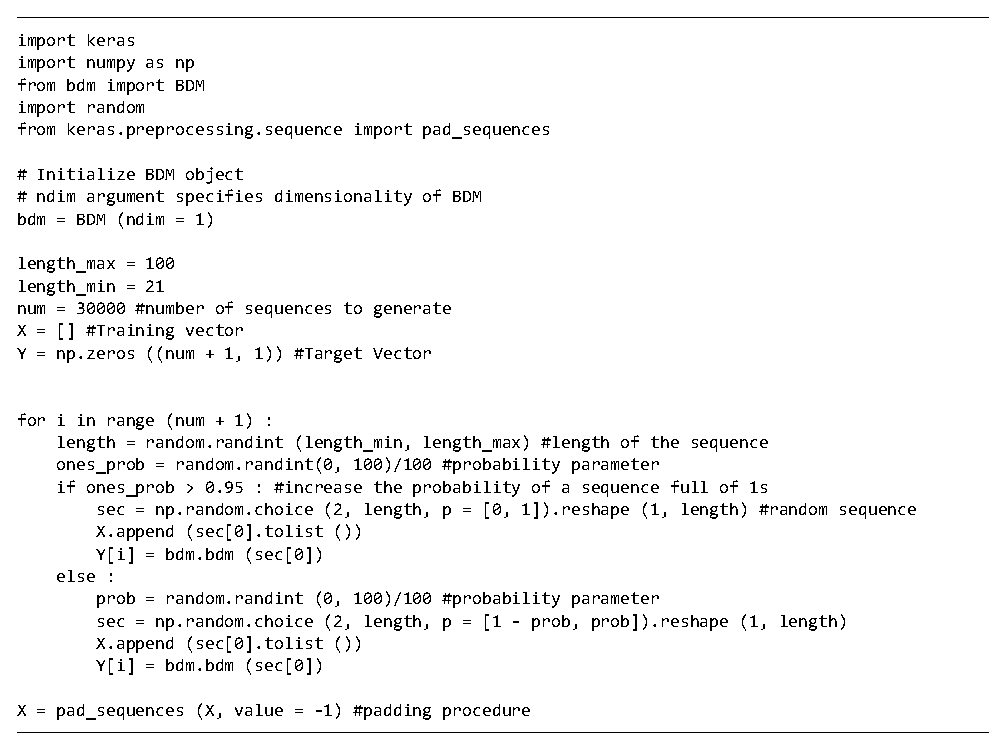
\includegraphics[width=\linewidth, height=\textheight,keepaspectratio]{training_data}
	\caption{The code to generate training data for the Neural Network which predicts Kolmogorov complexity.}
	\label{fig:training_data}
\end{figure}

\begin{figure}[h]
	\centering
		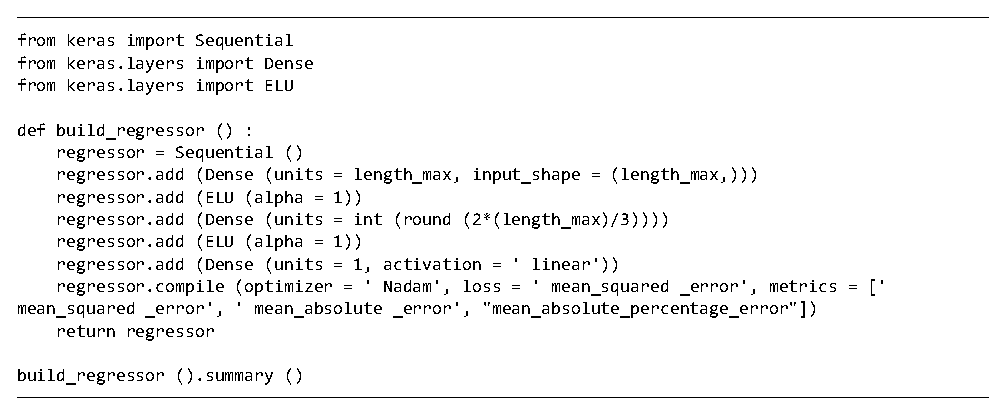
\includegraphics[width=\linewidth, height=\textheight,keepaspectratio]{nn_design_code}
	\caption{The code to build with the library Keras a Neural Network to perform regression.}
	\label{fig:nn_design_code}
\end{figure}

\begin{figure}[h]
	\centering
		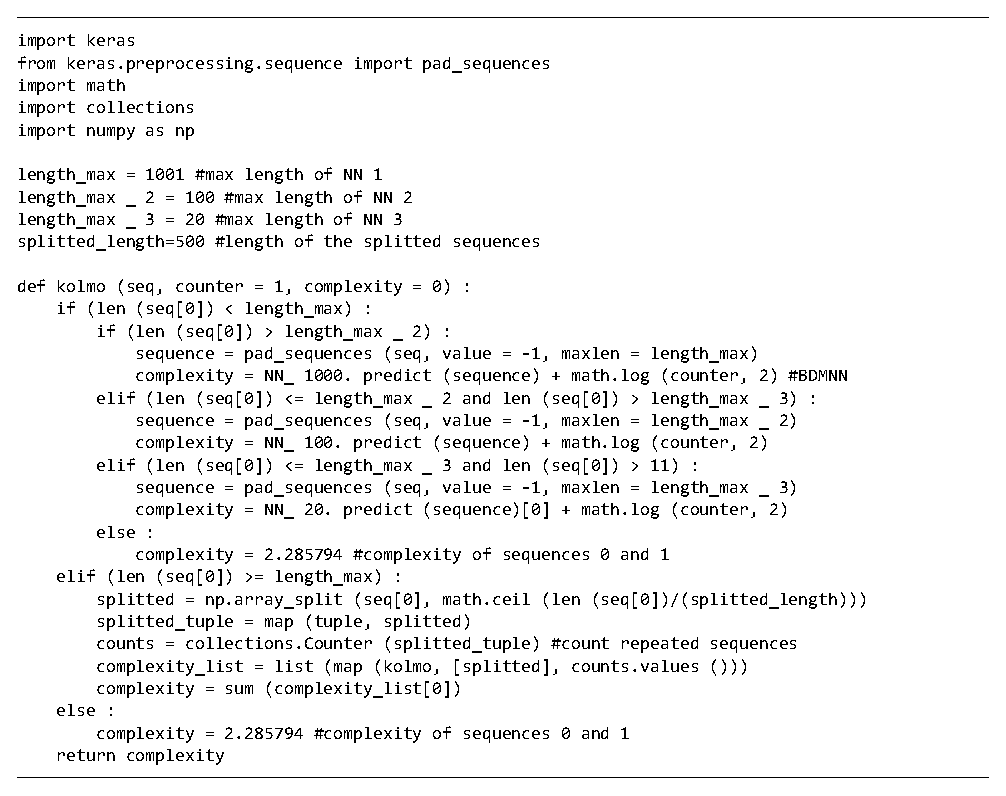
\includegraphics[width=\linewidth, height=\textheight,keepaspectratio]{def_fun_kolmo_code}
	\caption[The code to define a function which takes advantage of three Neural Network models to predict the K-complexity of sequences of any length.]{The code to define a function which takes advantage of three Neural Network models to predict the K-complexity of sequences of any length. The functions $NN \_20$, $NN \_100$, and $NN \_1000$ are the Neural Networks trained to predict the complexity of sequences in the corresponding interval of lengths.}
	\label{fig:def_fun_kolmo_code}
\end{figure}

\begin{figure}[h]
	\centering
		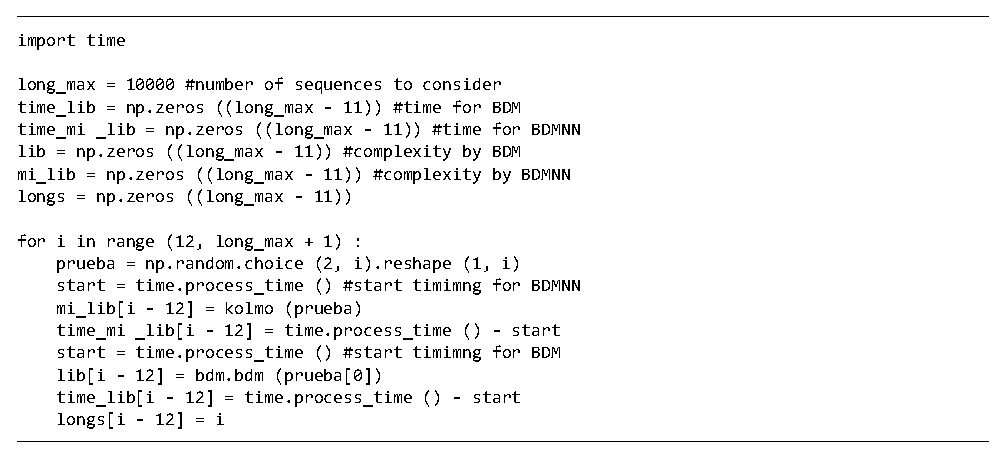
\includegraphics[width=\linewidth, height=\textheight,keepaspectratio]{timing_error_code}
	\caption{The code to perform the timing of the BDM and the BDMNN.}
	\label{fig:timing_error_code}
\end{figure}

\begin{figure}[h]
	\centering
		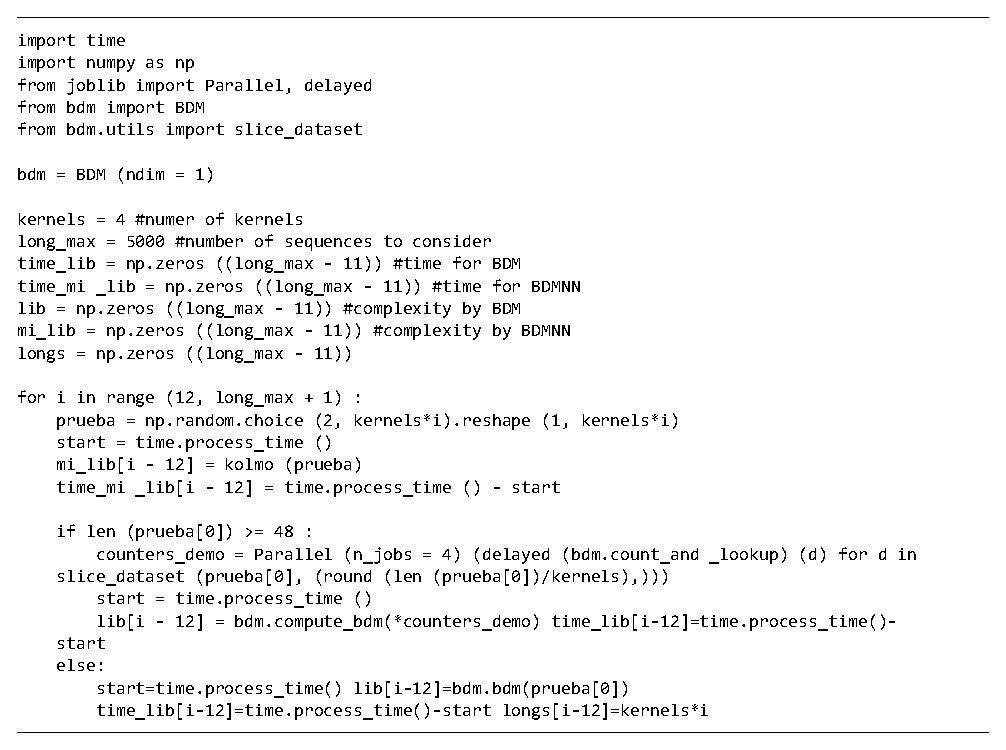
\includegraphics[width=\linewidth, height=\textheight,keepaspectratio]{timing_error_code_2}
	\caption[The code to perform the timing of the BDMNN and the parallel implementation of the BDM.]{The code to perform the timing of the BDMNN and the parallel implementation of the BDM. For the parallel implementation, it does not consider the time needed to split and distribute among the available kernels the given sequence. If we want to take into account this extra time we just need to move the line: $start = time.process \_ time()$ of the \textit{if} section, immediately before the declaration of $counters \_ demo$.}
	\label{fig:timing_error_code_2}
\end{figure}

